\section{Premises}

\begin{figure*}
	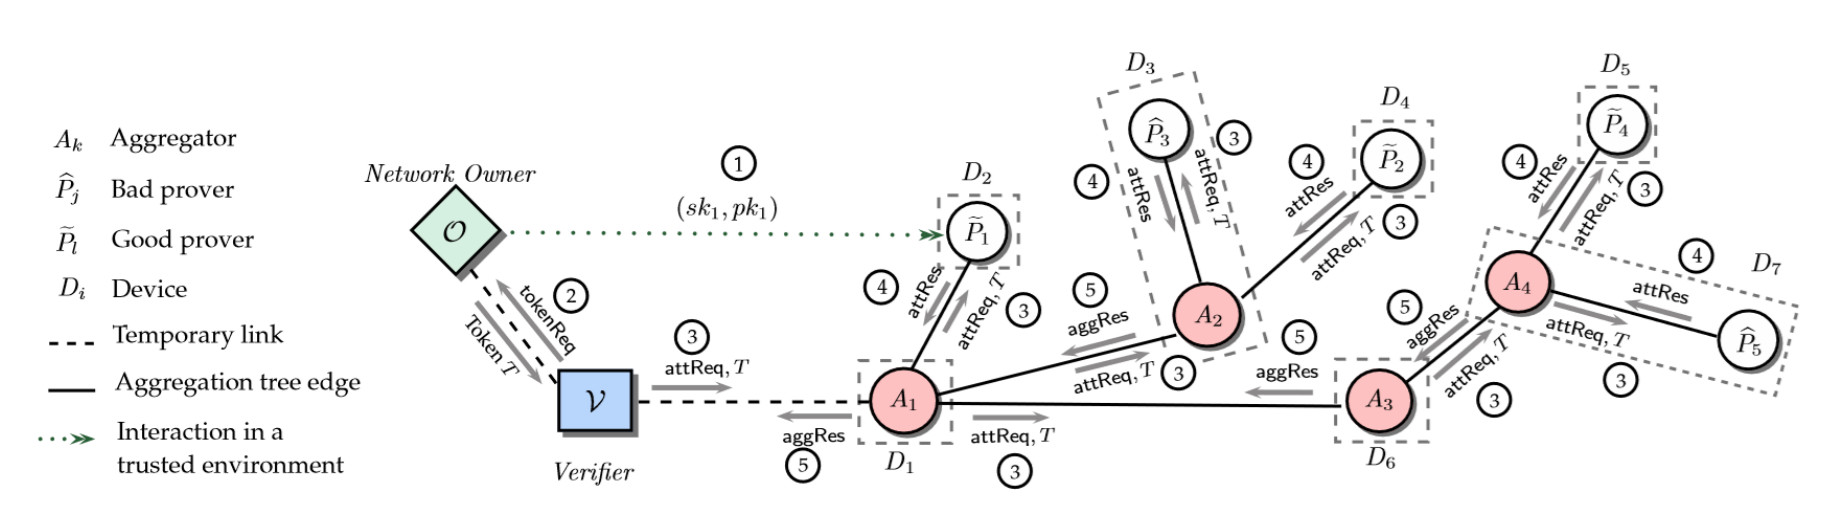
\includegraphics[width=0.9\linewidth]{Images/SANA_general.png} % Figure image
	\caption{Schematic of SANA propagation tree} % Figure caption
\end{figure*}

\subsection{Elliptic curve cryptography}
\todo{here just introduce ECC in general}
Elliptic Curve Cryptography (ECC) \todo{add citation.} is a public key
cryptographic method based on the algebraic structure of elliptic curves over
finite fields.
ECC security is based on the intractability of the elliptic
curve discrete logarithm problem.
In particular, it depends on the simplicity of computing a point multiplication 
on the curve as opposed to the intractability of computing the scalar multiplicand
given the original point and the result.
All this operations are performed with respect to the finite field the curve is associated with.

\subsection{SANA attestation protocol}
\todo{here introduce SANA propagation and how ECC is integrated in it.}
In SANA the remote attestation process starts from the verifier that sends a request to the Owner that generates a Token and propagates it to the Verifier (containing a challenge that will be proposed to the other nodes in order to certify the authenticity of the attestation request). The Verifier checks the signature and, if it has a positive result, stores the token. \\The Verifier then
the challenge to the closest Aggregator in the propagation tree, this node proceeds to propagate the challenge to its neighbours being other Aggregator
or Provers. The latter then sign a message according to their software configuration being legit or compromised. The signature travel back to the Aggregator
that creates the aggregated signature of its neighbours. Lastly the Verifier checks the aggregated signature of all the tree and determines which devices
can be trusted and which are compromised.\\
For implementing this protocol we chose an elliptic-curve implementation used in Ethereum and called ''bn128'' as it uses a Barreto-Naehrig curve and it's said to offer 128 bits security.
In SANA, the ECC is used to generate public keys that belong to a multiplicative
group that is composed by points on the curve we have chosen for the cryptrographic system.
After that all the signatures are generated by a random oracle as points belonging to the curve. We then use a fancy property of Elliptic curve to perform a bilinear function (called also pairing) on the signature received and a reconstruction of what should be the signature to check if it's authentic in a computationally efficient way.